\documentclass[]{article}
\usepackage{lmodern}
\usepackage{amssymb,amsmath}
\usepackage{graphicx}
\usepackage[final]{pdfpages}
\usepackage{ifxetex,ifluatex}
\usepackage{fixltx2e} % provides \textsubscript
\ifnum 0\ifxetex 1\fi\ifluatex 1\fi=0 % if pdftex
  \usepackage[T1]{fontenc}
  \usepackage[utf8]{inputenc}
\else % if luatex or xelatex
  \ifxetex
    \usepackage{mathspec}
  \else
    \usepackage{fontspec}
  \fi
  \defaultfontfeatures{Ligatures=TeX,Scale=MatchLowercase}
\fi
% use upquote if available, for straight quotes in verbatim environments
\IfFileExists{upquote.sty}{\usepackage{upquote}}{}
% use microtype if available
\IfFileExists{microtype.sty}{%
\usepackage{microtype}
\UseMicrotypeSet[protrusion]{basicmath} % disable protrusion for tt fonts
}{}
\usepackage{hyperref}
\hypersetup{unicode=true,
            pdftitle={Homework 3},
            pdfborder={0 0 0},
            breaklinks=true}
\urlstyle{same}  % don't use monospace font for urls
\IfFileExists{parskip.sty}{%
\usepackage{parskip}
}{% else
\setlength{\parindent}{0pt}
\setlength{\parskip}{6pt plus 2pt minus 1pt}
}
\setlength{\emergencystretch}{3em}  % prevent overfull lines
\providecommand{\tightlist}{%
  \setlength{\itemsep}{0pt}\setlength{\parskip}{0pt}}
\setcounter{secnumdepth}{0}
% Redefines (sub)paragraphs to behave more like sections
\ifx\paragraph\undefined\else
\let\oldparagraph\paragraph
\renewcommand{\paragraph}[1]{\oldparagraph{#1}\mbox{}}
\fi
\ifx\subparagraph\undefined\else
\let\oldsubparagraph\subparagraph
\renewcommand{\subparagraph}[1]{\oldsubparagraph{#1}\mbox{}}
\fi

\title{Homework 3}

\usepackage{geometry}
\geometry{letterpaper,textwidth=350pt,textheight=680pt,tmargin=60pt,
            left=72pt,footskip=24pt,headsep=18pt,headheight=14pt}
\usepackage{amsmath}
\usepackage{amssymb}
\usepackage{textcase}
\usepackage{soul}

\newcommand{\mat}[1]{\boldsymbol{#1}}
\renewcommand{\vec}[1]{\boldsymbol{\mathrm{#1}}}
\newcommand{\vecalt}[1]{\boldsymbol{#1}}

\newcommand{\conj}[1]{\overline{#1}}

\newcommand{\normof}[1]{\|#1\|}
\newcommand{\onormof}[2]{\|#1\|_{#2}}

\newcommand{\itr}[2]{#1^{(#2)}}
\newcommand{\itn}[1]{^{(#1)}}

\newcommand{\eps}{\varepsilon}
\newcommand{\kron}{\otimes}

\DeclareMathOperator{\diag}{diag}
\DeclareMathOperator{\trace}{trace}
\DeclareMathOperator{\tvec}{vec}

\newcommand{\prob}{\mathbb{P}}
\newcommand{\probof}[1]{\prob\left\{ #1 \right\}}

\newcommand{\pmat}[1]{\begin{pmatrix} #1 \end{pmatrix}}
\newcommand{\bmat}[1]{\begin{bmatrix} #1 \end{bmatrix}}
\newcommand{\spmat}[1]{\left(\begin{smallmatrix} #1 \end{smallmatrix}\right)}
\newcommand{\sbmat}[1]{\left[\begin{smallmatrix} #1 \end{smallmatrix}\right]}

\newcommand{\RR}{\mathbb{R}}
\newcommand{\CC}{\mathbb{C}}

\providecommand{\eye}{\mat{I}}
\providecommand{\mA}{\ensuremath{\mat{A}}}
\providecommand{\mB}{\ensuremath{\mat{B}}}
\providecommand{\mC}{\ensuremath{\mat{C}}}
\providecommand{\mD}{\ensuremath{\mat{D}}}
\providecommand{\mE}{\ensuremath{\mat{E}}}
\providecommand{\mF}{\ensuremath{\mat{F}}}
\providecommand{\mG}{\ensuremath{\mat{G}}}
\providecommand{\mH}{\ensuremath{\mat{H}}}
\providecommand{\mI}{\ensuremath{\mat{I}}}
\providecommand{\mJ}{\ensuremath{\mat{J}}}
\providecommand{\mK}{\ensuremath{\mat{K}}}
\providecommand{\mL}{\ensuremath{\mat{L}}}
\providecommand{\mM}{\ensuremath{\mat{M}}}
\providecommand{\mN}{\ensuremath{\mat{N}}}
\providecommand{\mO}{\ensuremath{\mat{O}}}
\providecommand{\mP}{\ensuremath{\mat{P}}}
\providecommand{\mQ}{\ensuremath{\mat{Q}}}
\providecommand{\mR}{\ensuremath{\mat{R}}}
\providecommand{\mS}{\ensuremath{\mat{S}}}
\providecommand{\mT}{\ensuremath{\mat{T}}}
\providecommand{\mU}{\ensuremath{\mat{U}}}
\providecommand{\mV}{\ensuremath{\mat{V}}}
\providecommand{\mW}{\ensuremath{\mat{W}}}
\providecommand{\mX}{\ensuremath{\mat{X}}}
\providecommand{\mY}{\ensuremath{\mat{Y}}}
\providecommand{\mZ}{\ensuremath{\mat{Z}}}
\providecommand{\mLambda}{\ensuremath{\mat{\Lambda}}}
\providecommand{\mPbar}{\bar{\mP}}

\providecommand{\ones}{\vec{e}}
\providecommand{\va}{\ensuremath{\vec{a}}}
\providecommand{\vb}{\ensuremath{\vec{b}}}
\providecommand{\vc}{\ensuremath{\vec{c}}}
\providecommand{\vd}{\ensuremath{\vec{d}}}
\providecommand{\ve}{\ensuremath{\vec{e}}}
\providecommand{\vf}{\ensuremath{\vec{f}}}
\providecommand{\vg}{\ensuremath{\vec{g}}}
\providecommand{\vh}{\ensuremath{\vec{h}}}
\providecommand{\vi}{\ensuremath{\vec{i}}}
\providecommand{\vj}{\ensuremath{\vec{j}}}
\providecommand{\vk}{\ensuremath{\vec{k}}}
\providecommand{\vl}{\ensuremath{\vec{l}}}
\providecommand{\vm}{\ensuremath{\vec{l}}}
\providecommand{\vn}{\ensuremath{\vec{n}}}
\providecommand{\vo}{\ensuremath{\vec{o}}}
\providecommand{\vp}{\ensuremath{\vec{p}}}
\providecommand{\vq}{\ensuremath{\vec{q}}}
\providecommand{\vr}{\ensuremath{\vec{r}}}
\providecommand{\vs}{\ensuremath{\vec{s}}}
\providecommand{\vt}{\ensuremath{\vec{t}}}
\providecommand{\vu}{\ensuremath{\vec{u}}}
\providecommand{\vv}{\ensuremath{\vec{v}}}
\providecommand{\vw}{\ensuremath{\vec{w}}}
\providecommand{\vx}{\ensuremath{\vec{x}}}
\providecommand{\vy}{\ensuremath{\vec{y}}}
\providecommand{\vz}{\ensuremath{\vec{z}}}
\providecommand{\vpi}{\ensuremath{\vecalt{\pi}}}

\sodef\allcapsspacing{\upshape}{0.15em}{0.65em}{0.6em}%

\makeatletter
\def\maketitle{%
\par
\hrule height 0.75pt\vspace{1ex}
\par\noindent
\begin{minipage}{0.5\textwidth}
\scshape
purdue university $\cdot$ cs 51400 \\
numerical analysis
\end{minipage}
\begin{minipage}{0.5\textwidth}
\raggedleft
\MakeTextUppercase{\allcapsspacing{\@title}}\\[0.2ex]
\textit{\@author}\\[0.2ex]
\textit{\@date}
\end{minipage}
\par\vspace{1ex}
\hrule height 1pt
\vspace{2ex}
\par
}
\makeatother

\author{Patrick Talley}
\title{Lecture Notes}
% auto generate a title
% \AtBeginDocument{\maketitle}

\title{Homework}



\begin{document}
\maketitle

Please answer the following questions in complete sentences in submit
the solution on Blackboard Fri. Sept. 30th by Midnight.

\section{Homework 3}\label{homework-3}

\begin{itemize}
\tightlist
\item
  2016-09-27: Small clarifications based on Piazza questions.
\end{itemize}

\subsection{Problem 1: Warm up problems (15
points)}\label{problem-1-warm-up-problems-15-points}

These questions are most similar to what I'd ask on an exam or on future
quizzes.

\begin{enumerate}
\def\labelenumi{\arabic{enumi}.}
\item
  Suppose \(\mA\) is an \(r \times s\) matrix. How many multiplication
  and addition operations are required for a general matrix vector
  product \(\mA \vx\).
\item
  Suppose \(\mA\) is an \(m \times n\) matrix and \(\mD\) is an
  \(m \times m\) diagonal matrix (that means that it has zeros
  everywhere except on the diagonal elements). Write down the simplest
  expression for the \(ij\)th entry of \(\mD \mA\) you can. (This will
  end up being used in the future for some problems!)
\item
  This is just like the previous problem, but now do the same thing
  where \(\mA\) is an \(m \times n\) matrix and \(\mD\) is an
  \(n \times n\) diagonal matrix. Write down the simplest expression for
  the \(ij\)th entry of \(\mA \mD\).
\end{enumerate}

%%% Solution start %%%
\textbf{Solution} 
\begin{enumerate}
\def\labelenumi{\arabic{enumi}.}
\item
\[ y_{ij} = \sum_{j=1}^{s} A_{ij}*x_{j} \] \\
This is done r times to form an r x 1 matrix. This means addition and multiplication is done $r*s$ times.
\item
\[ DA = C \in \mathbb{R}^{m*n}\]
\[ C_{ij} = D_{ii}A_{ij} \]
\item
\[ AD = C \in \mathbb{R}^{m*n}\]
\[ C_{ij} = D_{jj}A_{ij} \]
\end{enumerate}
%%% Solution end %%%

\subsection{Problem 2: Implement
MatMul}\label{problem-2-implement-matmul}

(If you wish, you may perform this task in a language besides Julia that
provides a built-in matrix-matrix multiplication routine -- such as
Matlab or Python, but you must have the same comparison.)

\begin{enumerate}
\def\labelenumi{\arabic{enumi}.}
\item
  Implement the following function:

\begin{verbatim}
"""
`matmul`
========

Compute Matrix-matrix multiplication or MatMul.

Functions
---------
- `C = matmul(A,B)` returns the matrix-matrix product of C=A*B
"""
function matmul(A,B)        
end
\end{verbatim}

  using only scalar operations. (i.e.~without any of Julia's built in
  matrix operations.)
\item
  Report the output of your function for the following commands

\begin{verbatim}
@show matmul([1 2], [2; 1])
@show matmul([1 2; -2 4; 0 3], [-1; 1])
@show matmul([-1 1], [1 -2 0; 2 4 3])
@show matmul(3, 5)
t = pi/2
@show matmul([cos(t) -sin(t); sin(t) cos(t)], 
    [cos(t) sin(t); -sin(t) cos(t)]);
\end{verbatim}
\item
  Compare the time and accuracy of your code to Julia's built in
  matrix-matrix operator \texttt{*} on matrices of random normals with
  sizes ranging between \(10\) and \(1000\). To evaluate accuracy, use:

\begin{verbatim}
C = matmul(A,B)
D = A*B
diff = vecnorm(C-D,);
\end{verbatim}

  To evaluate time, use:

\begin{verbatim}
dt = @elapsed C = matmul(A,B);
\end{verbatim}

  Use 50 different random samples for each size and report the mean time
  for Julia vs.~your own code as one plot. (So on the x-axis we have
  problem size, and on the y axis, we have one line for the mean time
  over 50 trials of Julia's built-in operation, and a second line we
  have the mean time over 50 trials of our function.)

  Also prepare the same type of plot on the \emph{maximum difference}
  over 50 trials between your code and Julia's code to show the
  accuracy.
\item
  Write a new function:

\begin{verbatim}
"""
`matmul2`
========

Compute Matrix-matrix multiplication or MatMul faster

Functions
---------
- `C = matmul(A,B)` returns the matrix-matrix product of C=A*B
"""
function matmul(A,B)        
end
\end{verbatim}

  That uses some of the ideas we talked about in class to make a faster
  matrix-matrix product. You may use Julia's built-in matrix-matrix
  multiplication for up to 16-by-16 matrices. Or matrix-vector products
  up to \(256-by-1\). Compare the time and accuracy of your new
  \texttt{matmul2} code to your original.
\end{enumerate}

%%% Solution start %%%
\textbf{Solution} 
\begin{enumerate}
\def\labelenumi{\arabic{enumi}.}
\item

\item
matmul([1 2],[2;1]) = [4.0] \\
matmul([1 2;-2 4;0 3],[-1;1]) = 
\[ \begin{bmatrix}1.0 \\ 6.0 \\ 3.0
\end{bmatrix} \] 
matmul([-1 1],[1 -2 0;2 4 3]) = [1.0 6.0 3.0] \\
matmul(3,5) = [15.0] \\
matmul([cos(t) -(sin(t));sin(t) cos(t)],[cos(t) sin(t);-(sin(t)) cos(t)]) = 
\[ \begin{bmatrix}1.0 & 0.0 \\
0.0&1.0]
\end{bmatrix} \]
\item
\hfill \break
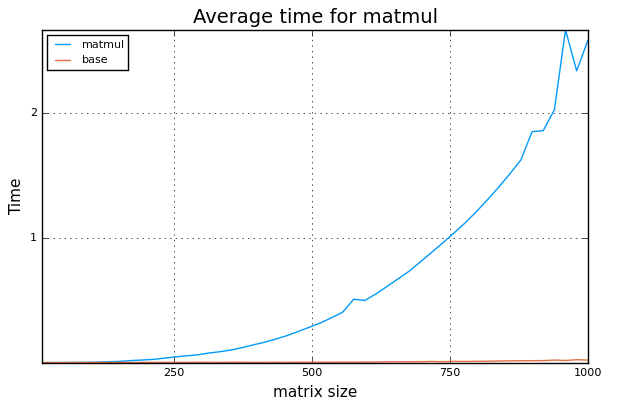
\includegraphics[width=\textwidth,keepaspectratio]{problem2partB.png}
\hfill \break
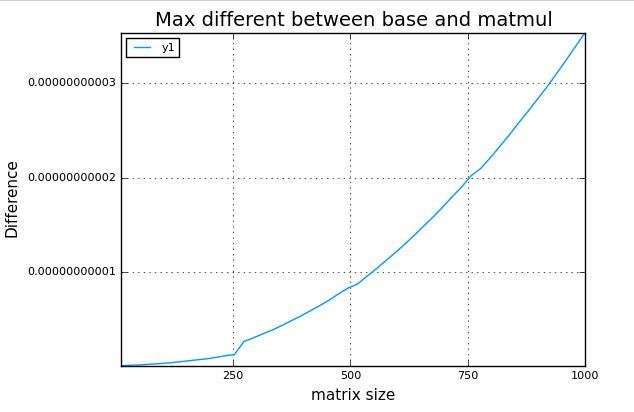
\includegraphics[width=\textwidth,keepaspectratio]{problem2partC.png}
\item

\item
\hfill \break
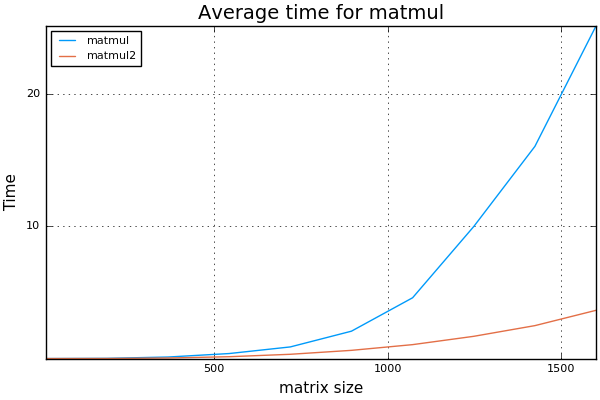
\includegraphics[width=\textwidth,keepaspectratio]{problem2partD.png}
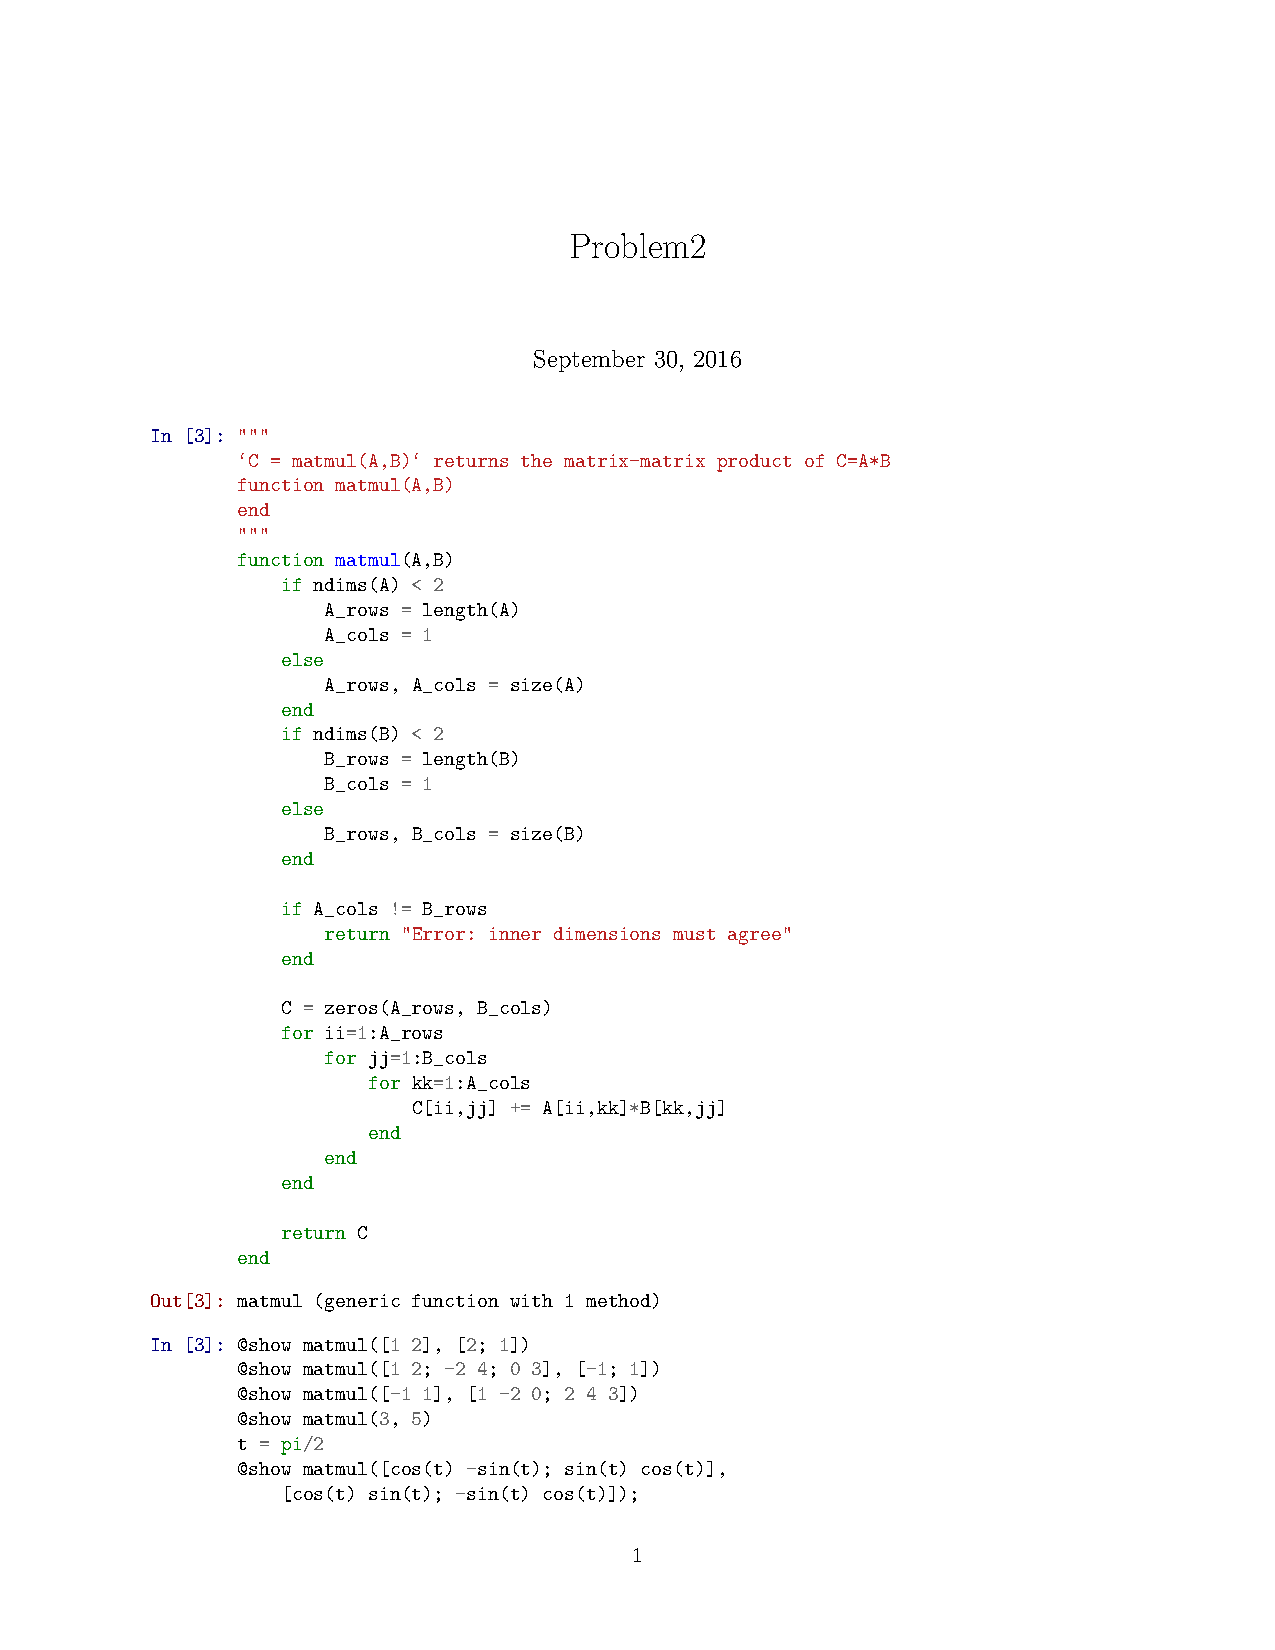
\includepdf[pages=-]{Problem2.pdf}
\end{enumerate}
%%% Solution end %%%

\subsection{Problem 3: Make Yoda Spin!}\label{problem-3-make-yoda-spin}

\begin{enumerate}
\def\labelenumi{\arabic{enumi}.}
\item
  G\&C Chapter 2 Problem 11. The Julia code for this example is

\begin{verbatim}
# create matrix whose columns contain the coordinates of
# each vertex.
U = [1.0 0 -1 0 1.0; 0 1 0 -1 0]

theta = pi/4.0

# Create a red unit square
# Note U(1,:) denotes the first row of U
plot(U[1,:]',U[2,:]',fill=(0,:red))

# Perform rotation.
R = [cos(theta) -sin(theta); sin(theta) cos(theta)];
V = R*U;
# Plot the blue square
plot!(V[1,:]', V[2,:]',fill=(0,:blue))
\end{verbatim}
\item
  G\&C Chapter 2 Problem 12 (not assigned)

\begin{verbatim}
**I really wanted to assign this one, but I still haven't 
figured out how to translate the Matlab code into Julia
code. This one might get assigned in the future.**
\end{verbatim}
\end{enumerate}

%%% Solution start %%%
\textbf{Solution} 
\hfill \break
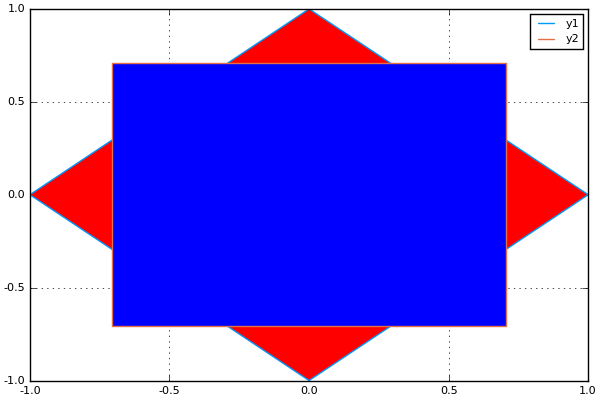
\includegraphics[width=\textwidth,keepaspectratio]{problem3.png}
\begin{enumerate}
\def\labelenumi{\arabic{enumi}.}
\item
\hfill \break
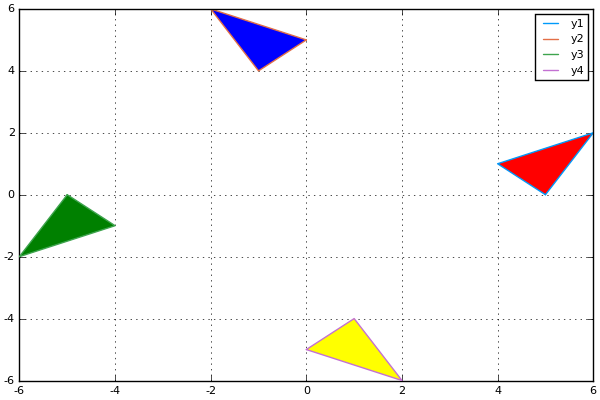
\includegraphics[width=\textwidth,keepaspectratio]{problem3partA.png}
\item
\hfill \break
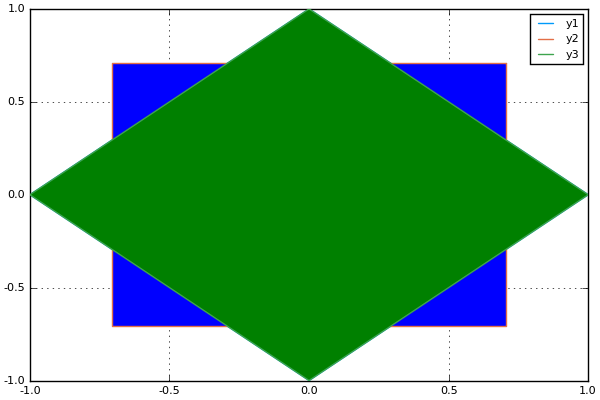
\includegraphics[width=\textwidth,keepaspectratio]{problem3partB.png}
\item
\[ R(\theta) * R(-\theta) = \begin{bmatrix} 
cos^2\theta + sin^2\theta & cos\theta sin\theta - cos\theta sin\theta \\
cos\theta sin\theta - cos\theta sin\theta & cos^2\theta + sin^2\theta
\end{bmatrix} = \begin{bmatrix} 
1 & 0 \\
0 & 1
\end{bmatrix}
\]
\item
\hfill \break
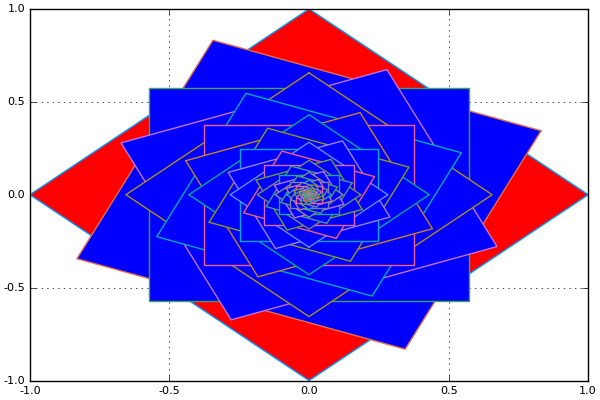
\includegraphics[width=\textwidth,keepaspectratio]{problem3partC.png}
\item
\hfill \break
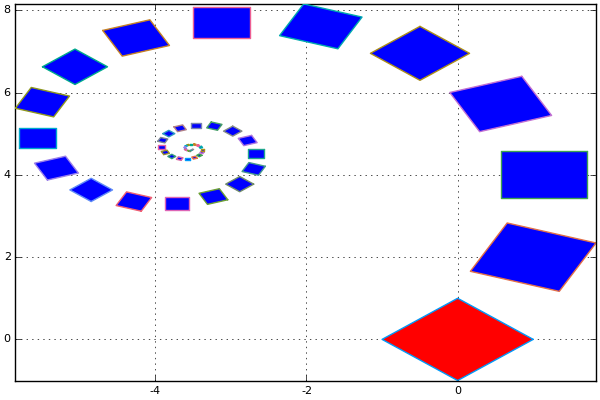
\includegraphics[width=\textwidth,keepaspectratio]{problem3partD.png}
\end{enumerate}
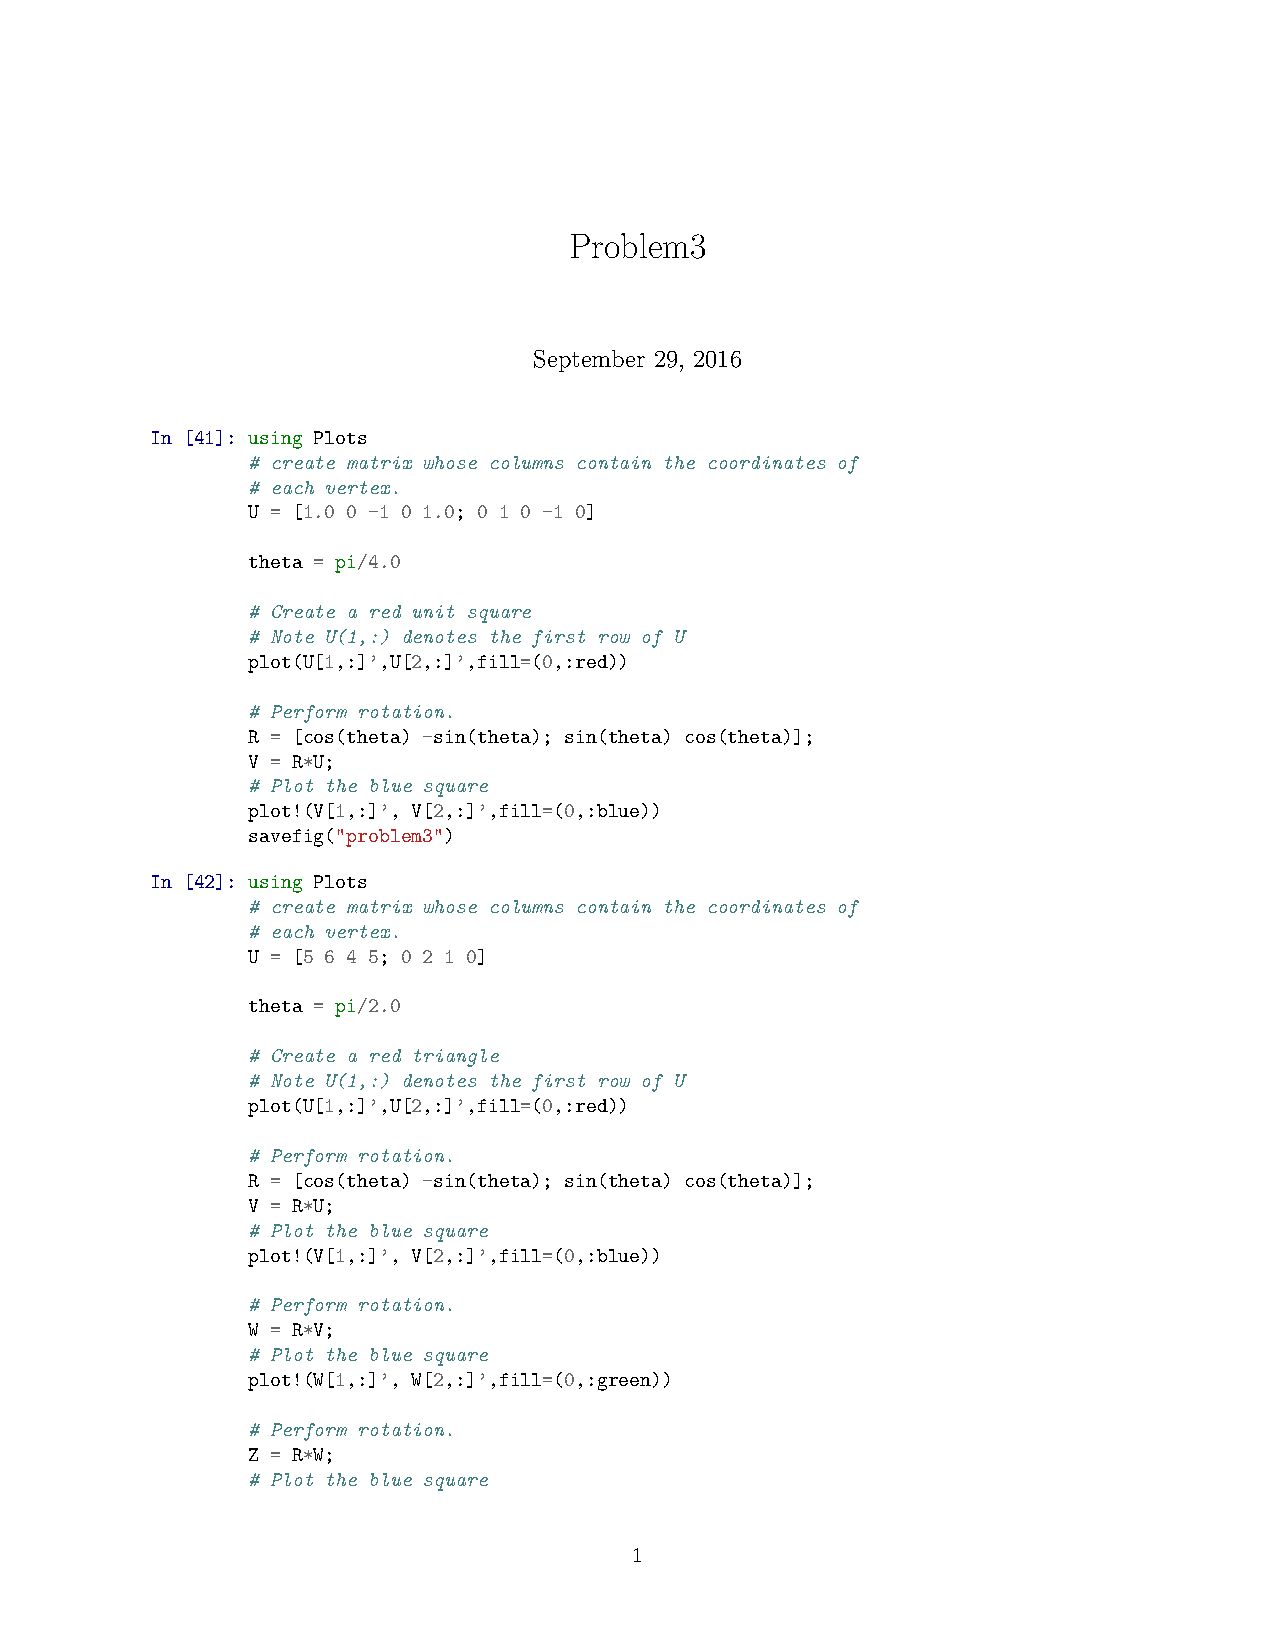
\includepdf[pages=-]{Problem3.pdf}

%%% Solution end %%%

\subsection{Problem 4: Make an image
small}\label{problem-4-make-an-image-small}

Consider the following problem. We have a \(32 \times 32\) pixel image.
Each pixel is a real-valued number between \(0\) and \(1\). However, I
want to show this on an iPhone and I only have a \(16 \times 16\) pixel
area to show the image. In order to reduce the size of the image, I want
to average groups of 4 pixels. In this problem, we'll create a Julia
program to do this

Let's work through a smaller example first. For the \(4 \times 4\)
image, represented here by a matrix-like array:
\[ \bmat{ x_{1} & x_2 & x_3 & x_4 \\
          x_5 & x_6 & x_7 & x_8 \\
          x_9 & x_{10} & x_{11} & x_{12} \\
          x_{13} & x_{14} & x_{15} & x_{16} }  \] I want to compute
\[ \bmat{ (x_1 + x_2 + x_5 + x_6)/4 & (x_3 + x_4 + x_7 + x_8)/4 \\
   (x_9 + x_{10} + x_{13} + x_{14})/4 & (x_{11} + x_{12} + x_{15} + x_{16})/4 }. \]

We will solve this problem using a matrix-vector product.

\begin{enumerate}
\def\labelenumi{\arabic{enumi}.}
\item
  Suppose I call:

  \[ \begin{matrix} 
     y_1 = (x_1 + x_2 + x_5 + x_6)/4 & y_2 = (x_3 + x_4 + x_7 + x_8)/4 \\
     y_3 = (x_9 + x_{10} + x_{13} + x_{14})/4 & y_4 = (x_{11} + x_{12} + x_{15} + x_{16})/4. \end{matrix} \]

  Further, suppose we consider the vectors \(\vy \in \RR^{4}\) and
  \(\vx \in \RR^{16}\) to be the new image and old image, respectively.
  Write down the matrix \(\mA\) such that \(\vy = \mA \vx\).

  \textbf{In the remainder of the problem, we'll work through how to do
  this for a particular image in Julia. }
\item
  Download
  \url{http://www.cs.purdue.edu/homes/dgleich/cs314-2016/homeworks/smallicon.csv}
  and type

\begin{verbatim}
download("http://www.cs.purdue.edu/homes/dgleich/cs314-2016/homeworks/smallicon.csv","smallicon.csv")
X = readcsv("smallicon.csv")
\end{verbatim}

  in Julia. You should get a \(32 \times 32\) matrix \(\mX\). What is
  the sum of diagonal elements of \(\mX\)?
\item
  Show the image

\begin{verbatim}
using Images
grayim(X)
\end{verbatim}

  Or write it to a file

\begin{verbatim}
using FileIO
using ImageMagick
save("icon1.png",X)
\end{verbatim}

  But that picture doesn't look right, does it? To get full points, make
  sure you adjust the figure so that it looks correct.!

  Show your final code and the image you get.
\item
  In what follows, we'll talk about two different types of indices. The
  image index of a pixel is a pair \((i,j)\) that identifies a row and
  column for the pixel in the image. The vector index of a pixel is the
  index of that pixel in a linear ordering of the image elements. For
  instance, in the small little example, pixel (3,2) has linear index
  \(10\). Also, pixel (1,4) has index \(4\). Julia can help us built a
  map between pixel indices and linear or vector indices:

\begin{verbatim}
N = reshape(1:(4*4), 4, 4)'
\end{verbatim}

  This creates the pixel index to linear index for the problem above
  because

\begin{verbatim}
N(1,4) 
N(3,2)
\end{verbatim}

  return the appropriate entry.

  In your own words, explain what the \texttt{reshape} operation does.
  What happens if you omit the final transpose above and try:

\begin{verbatim}
N = reshape(1:(4*4), 4, 4)
\end{verbatim}

  instead?
\item
  Now we need to construct the matrix \(\mA\) in order to reduce the
  size of a \(32 \times 32\) image to a \(16 \times 16\) image as we did
  in part 1.\\
  Suppose we call the output vector \(\vy\) and the output image
  \(\mY\). I'm giving you the following template, that I hope you can
  fill in. Feel free to construct an \(\mA\) that accomplishes our image
  reduction task any way you choose, but the following should provide
  some guidance.

\begin{verbatim}
NX = <fill in> # the map between pixel indices and linear indices for X
NY = <fill in> # the map between pixel indices and linear indices for Y
A = <fill in>  # the matrix we are trying to build
for i=1:32
    for j=1:32    
        xi = <fill in> # the index of the pixel i,j in the vector x
        yi = <fill in> # hint, div(i,k) is integer division!

        A[yi,xi] = 1/4 # place the entry of the matrix
    end
end
\end{verbatim}
\item
  In order to use the matrix \(\mA\) we created, we need to convert the
  matrix \(\mX\) into a vector! The reshape operation helps here:

\begin{verbatim}
x = reshape(X',32*32,1)
\end{verbatim}

  We can now rescale the image \(\mX\) by multiplying by \(\mA\) and
  reorganizing back into a matrix \(\mY\).

\begin{verbatim}
y = A*x
Y = reshape(y,16,16)'
\end{verbatim}

  Show the image of \(\mY\). Does that look correct?\\
  (Hint, apply the same correction you did before!)
\end{enumerate}

%%% Solution start %%%
\textbf{Solution} 
\begin{enumerate}
\def\labelenumi{\arabic{enumi}.}
\item
\item
\[ 24.36862745098039 \]
\item 
\hfill \break

\includegraphics[keepaspectratio]{problem4partA.png}
\item
Reshape will take the vector from 1-16 and place it into a 4x4 matrix by going down the columsn. If you ignore the transpose the first row would be 1 5 9 13 instead of 1 2 3 4. 
\item
\hfill \break

\includegraphics[keepaspectratio]{problem4partD.png}
\end{enumerate}
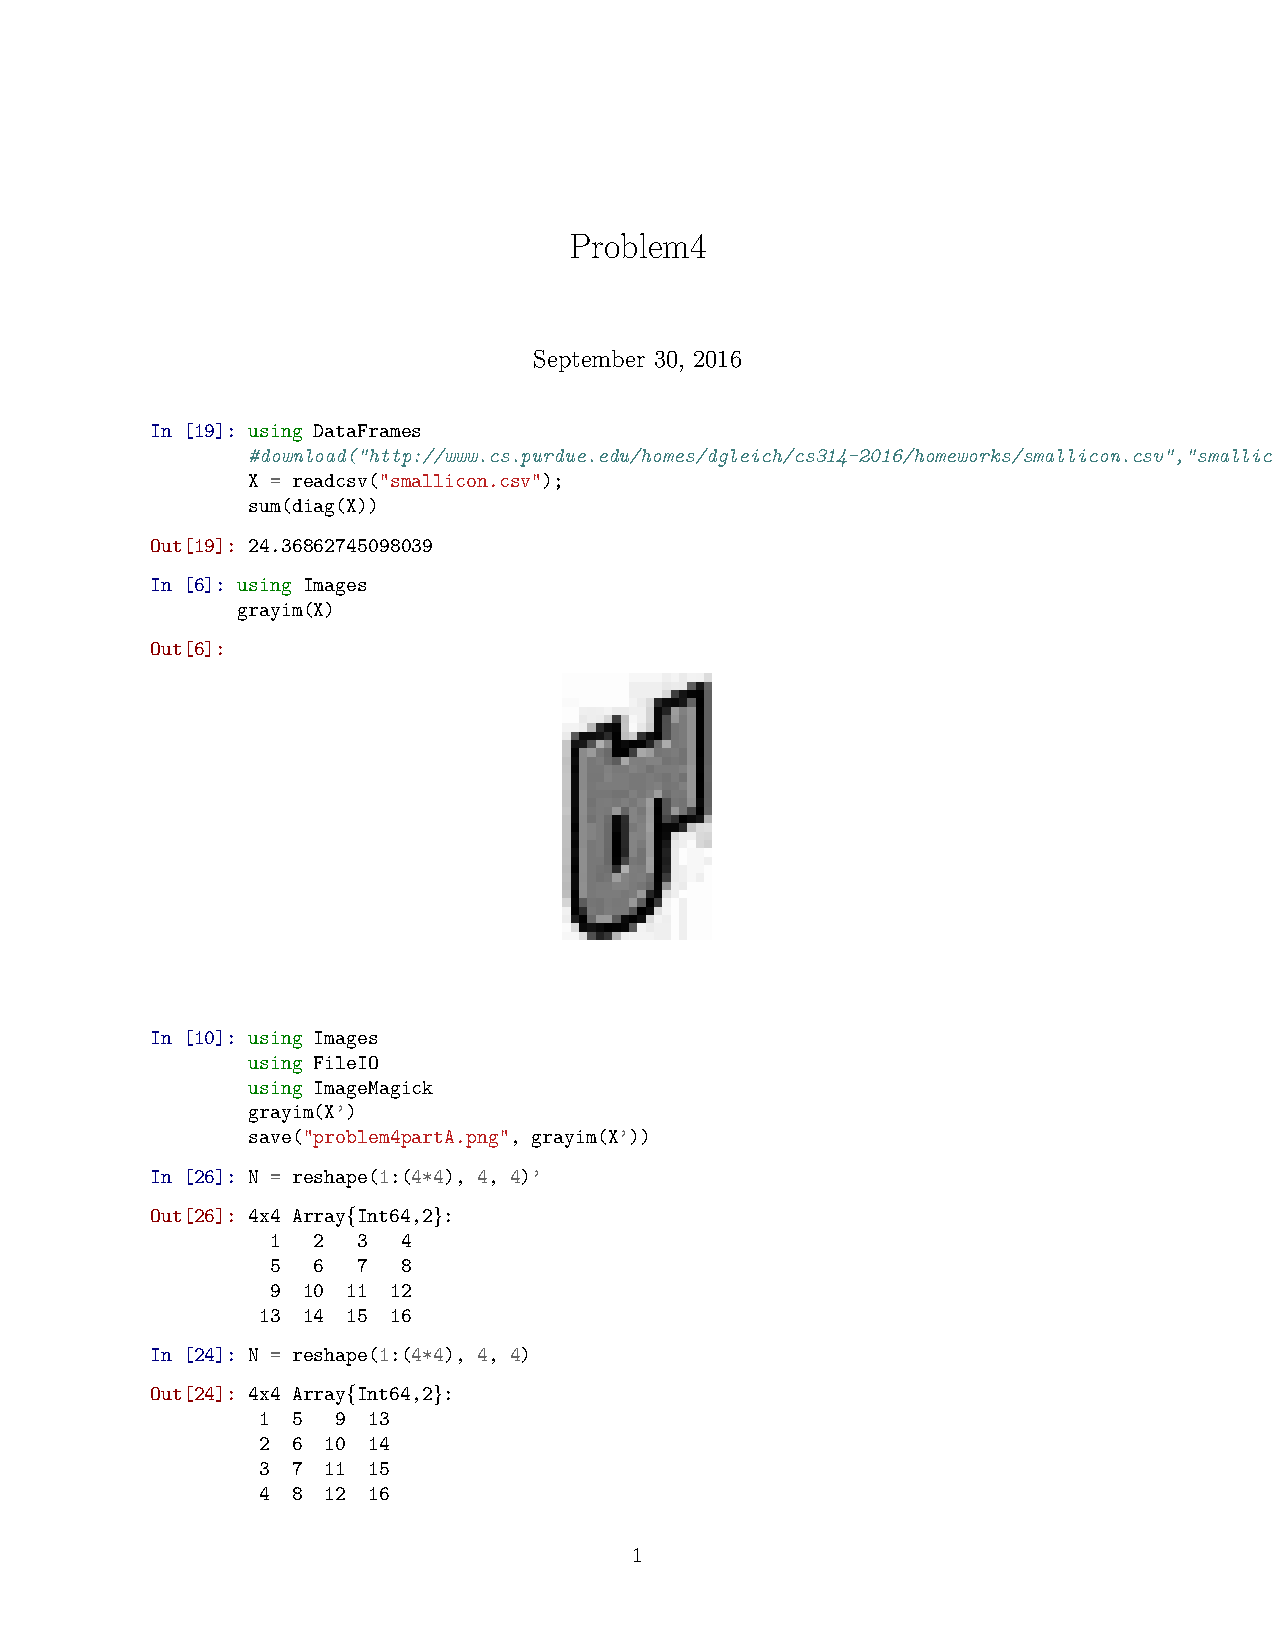
\includepdf[pages=-]{Problem4.pdf}
%%% Solution end %%%

\end{document}
